% Needed and Layout
\documentclass[a4paper,11pt]{article}
\usepackage[utf8]{inputenc} % utf8 encoding
\usepackage{amsfonts}
\usepackage[T1]{fontenc} % use for allowing < and > in cleartext
\usepackage[margin=2.5cm]{geometry}

% Lists
\usepackage{verbatim}   % useful for program listings
\usepackage{enumitem}
\usepackage[ampersand]{easylist}

% Creating more compact lists
\let\olditemize\itemize
\renewcommand{\itemize}{
    \olditemize
    \setlength{\itemsep}{1pt}
    \setlength{\parskip}{0pt}
    \setlength{\parsep}{0pt}
}



% Math
\usepackage{mathtools}   % need for subequations

% Graphics
\usepackage{graphicx}   % need for figures
\usepackage{color}      % use if color is used in text 
\usepackage{tikz}
\usetikzlibrary{arrows}
\usepackage{float}

% Other
\usepackage{url}
\usepackage{todonotes}
\usepackage{pdfpages}
\usepackage{subcaption}
\usepackage{latexsym}
\usepackage{fixltx2e}    % use for textsubscript
\usepackage[titletoc,title]{appendix}
\usepackage[framemethod=tikz]{mdframed}
\usepackage[titletoc,title]{appendix}
\usepackage{epstopdf}
\bibliographystyle{plain}

% Code listing
\usepackage{listings} % For inserting code from file (I think)
\usepackage{algorithm}
\usepackage{algpseudocode}
\renewcommand{\algorithmicforall}{\textbf{for each}}
\makeatletter
\def\BState{\State\hskip-\ALG@thistlm}
\makeatother

\DeclareCaptionFormat{algor}{%
  \hrulefill\par\offinterlineskip\vskip1pt%
    \textbf{#1#2}#3\offinterlineskip\hrulefill}
\DeclareCaptionStyle{algori}{singlelinecheck=off,format=algor,labelsep=space}
\captionsetup[algorithm]{style=algori}

% URLs ? maybe
\usepackage[hypcap=false]{caption}
\usepackage{hyperref}


% I wonder what this is
\definecolor{codegreen}{rgb}{0,0.6,0}
\definecolor{codegray}{rgb}{0.5,0.5,0.5}
\definecolor{codepurple}{rgb}{0.58,0,0.82}
\definecolor{backcolour}{rgb}{1.0,1.0,1.0}
\lstdefinestyle{mystyle}{
  backgroundcolor=\color{backcolour},   commentstyle=\color{codegreen},
  keywordstyle=\color{magenta},
  numberstyle=\tiny\color{codegray},
  stringstyle=\color{codepurple},
  basicstyle=\footnotesize,
  breakatwhitespace=false,         
  breaklines=true,                 
  captionpos=b,                    
  keepspaces=true,                 
  numbers=left,                    
  numbersep=5pt,                  
  showspaces=false,                
  showstringspaces=false,
  showtabs=false,                  
  tabsize=2
}
\lstset{style=mystyle}

\begin{document}

% Configuration
\setlength{\parindent}{0cm}
\setlength{\unitlength}{1mm}

% Front Page
\date{September 1st 2015\\ IT University of Copenhagen}
\title{A Quantitative Analysis of Bugs in Linux}
\author{Elvis Flesborg\\
\texttt{efle@itu.dk}}
\clearpage\maketitle
\thispagestyle{empty}
\newpage

%%%%%%%%%%%%%%%%%%%%%%%%%%%%%%%%%%%%%%%%%%%%%%%%%%%%%%%%%%%%%%%%%%%%%%%%%%%%%%%%
%                           TABLE OF CONTENTS
%%%%%%%%%%%%%%%%%%%%%%%%%%%%%%%%%%%%%%%%%%%%%%%%%%%%%%%%%%%%%%%%%%%%%%%%%%%%%%%%
\tableofcontents
\thispagestyle{empty}



\newpage

\setcounter{page}{1}

\section{Abstract}
\emph{---Leave blank until the end---}

\section{Introduction}
\emph{---Leave blank until the end---}




%%%%%%%%%%%%%%%%%%%%%%%%%%%%%%%%%%%%%%%%%%%%%%%%%%%%%%%%%%%%%%%%%%%%%%%%%%%%%%%%
%                           BACKGROUND
%%%%%%%%%%%%%%%%%%%%%%%%%%%%%%%%%%%%%%%%%%%%%%%%%%%%%%%%%%%%%%%%%%%%%%%%%%%%%%%%
\newpage
\section{Background}

\subsection{Linux}

The Linux kernel has around 11,000 features in the feature model. And further,
it is the largest open source codebase. This is great for testing purposes
regarding variability.

\begin{itemize}
    \item 11,000 features - how I found out.
    \item Open source
    \item Largest codebase
    \item linux-next
\end{itemize}

\subsection{Kconfig}

The Kconfig language is the language of the feature model in Linux (also for 
other projects like busybox, vim, etc...)

\begin{itemize}
    \item Explain the Kconfig language a bit
    \item Show a dependency tree
    \item Examples of constraints in the language
    \item Reference to Thorsten's projects
\end{itemize}

\subsection{randconfig}

\begin{itemize}
    \item Show some code
    \item Show a graph with a toy example
\end{itemize}

\subsection{gcc bugtypes}



%%%%%%%%%%%%%%%%%%%%%%%%%%%%%%%%%%%%%%%%%%%%%%%%%%%%%%%%%%%%%%%%%%%%%%%%%%%%%%%%
%                           METHODOLOGY
%%%%%%%%%%%%%%%%%%%%%%%%%%%%%%%%%%%%%%%%%%%%%%%%%%%%%%%%%%%%%%%%%%%%%%%%%%%%%%%%
\newpage
\section{Methodology}

\subsection{Research Questions}

\begin{itemize}
    \item How many of the possible configurations are valid
    \item Top Errors
    \item Top Subsystems with errors
    \item Top features with errors
    \item Difference between same version, and constantly updated version of 
        linux-next
\end{itemize}

\subsection{Collecting data}

\begin{itemize}
    \item Grepping the stderr
    \item Categorizing the warnings/Errors
    \item About the collection machine
    \item About the database setup
\end{itemize}




%%%%%%%%%%%%%%%%%%%%%%%%%%%%%%%%%%%%%%%%%%%%%%%%%%%%%%%%%%%%%%%%%%%%%%%%%%%%%%%%
%                                 DATA
%%%%%%%%%%%%%%%%%%%%%%%%%%%%%%%%%%%%%%%%%%%%%%%%%%%%%%%%%%%%%%%%%%%%%%%%%%%%%%%%
\newpage
\section{Data}

\begin{itemize}
    \item Example of data structure
    \item Graph of tables
\end{itemize}




%%%%%%%%%%%%%%%%%%%%%%%%%%%%%%%%%%%%%%%%%%%%%%%%%%%%%%%%%%%%%%%%%%%%%%%%%%%%%%%%
%                               RESULTS
%%%%%%%%%%%%%%%%%%%%%%%%%%%%%%%%%%%%%%%%%%%%%%%%%%%%%%%%%%%%%%%%%%%%%%%%%%%%%%%%
\newpage
\section{Results}

\subsection{Analyzing the data}

\subsection{Number of valid configurations}

\subsection{Observations}




%%%%%%%%%%%%%%%%%%%%%%%%%%%%%%%%%%%%%%%%%%%%%%%%%%%%%%%%%%%%%%%%%%%%%%%%%%%%%%%%
%                           THREATS TO VALIDITY
%%%%%%%%%%%%%%%%%%%%%%%%%%%%%%%%%%%%%%%%%%%%%%%%%%%%%%%%%%%%%%%%%%%%%%%%%%%%%%%%
\newpage
\section{Threats to Validity}

\subsection{Generate'n'Filter}

\begin{itemize}
    \item Uniform distribution
    \item Too low percentage
    \item Get a lower bound on the percentage
    \item sharpSAT?
\end{itemize}

\subsection{elvisconfig}

\begin{itemize}
    \item Maybe the permutation script can be used elsewhere (Thorsten seemed 
        interested)
\end{itemize}

\subsection{RandomSAT}





%%%%%%%%%%%%%%%%%%%%%%%%%%%%%%%%%%%%%%%%%%%%%%%%%%%%%%%%%%%%%%%%%%%%%%%%%%%%%%%%
%                           RELATED WORK
%%%%%%%%%%%%%%%%%%%%%%%%%%%%%%%%%%%%%%%%%%%%%%%%%%%%%%%%%%%%%%%%%%%%%%%%%%%%%%%%
\newpage
\section{Related Work}

\begin{itemize}
    \item 42 bugs
    \item Variability in ...
    \item Paper from Iago
    \item Fengguang Wu and Intel
\end{itemize}



\newpage
\section{Conclusion}
\emph{--- Leave empty until the end---}




\newpage
\bibliography{bibliography}

\end{document}

% Example of Bibliography
\newpage
\bibliography{bibliography}

% Example of Appendix
\begin{appendices}
\section{Code}
\lstinputlisting[language=Python]{../temp.py}
\end{appendices}

% Example of a drawing
\begin{figure}[H]
    \begin{center}
        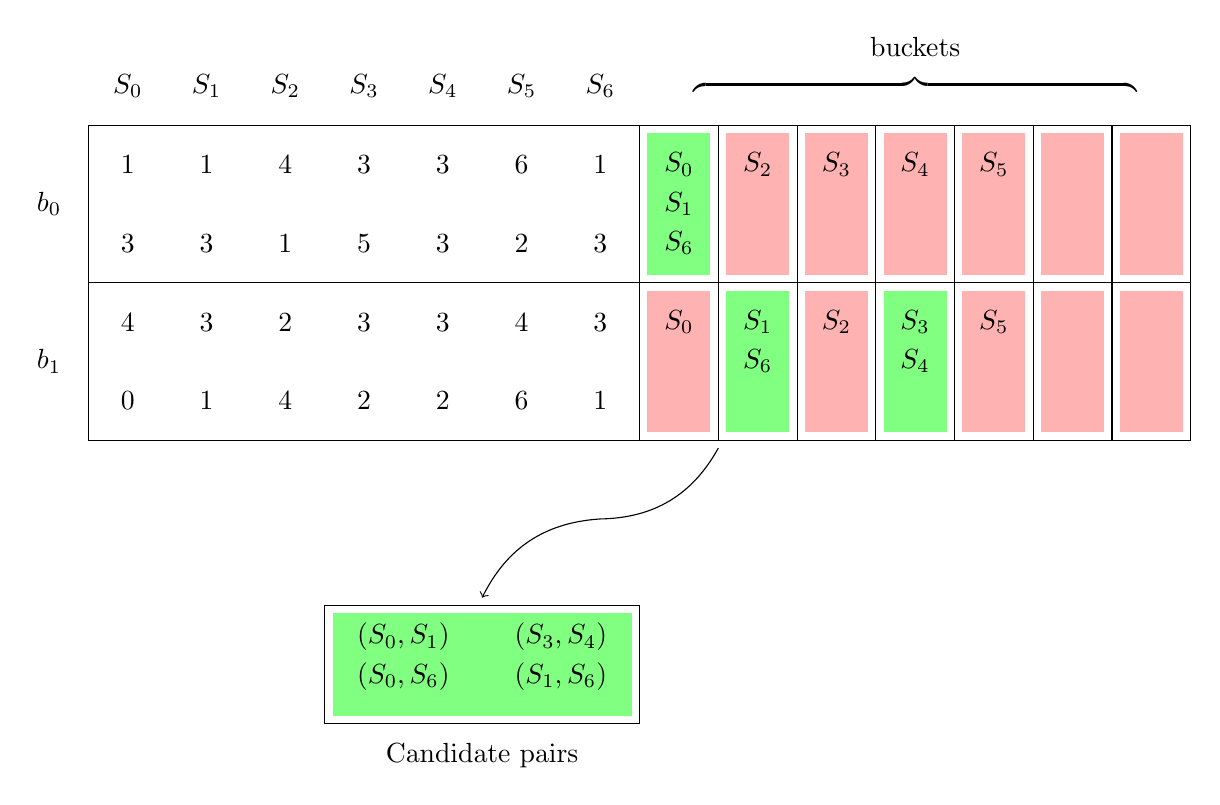
\begin{tikzpicture}
            \draw rectangle (14,4);
            \draw rectangle (7,2);
            \draw (0,2) rectangle (7,2);
            \draw (7,0) rectangle (8,4);

            \foreach \x in {0,...,6} \draw (\x+7, 0) rectangle (\x+7+1, 2);
            \foreach \x in {0,...,6} \draw (\x+7, 2) rectangle (\x+7+1, 4);
            \foreach \x in {0,...,6} \draw (\x+.5, 4.5) node {$S_\x$};

            \draw (-.5,3) node {$b_0$};
            \draw (-.5,1) node {$b_1$};

            % The overbrace
            \draw (10.5, 4.5) node {$\overbrace{\qquad\qquad\qquad\qquad\qquad\qquad\qquad\qquad}$};
            \draw (10.5,5.0) node {buckets};

            % Signature matrix (left part)
            \draw (0.5,3.5) node {1};
            \draw (0.5,2.5) node {3};
            \draw (0.5,1.5) node {4};
            \draw (0.5,0.5) node {0};

            \draw (1.5,3.5) node {1};
            \draw (1.5,2.5) node {3};
            \draw (1.5,1.5) node {3};
            \draw (1.5,0.5) node {1};

            \draw (2.5,3.5) node {4};
            \draw (2.5,2.5) node {1};
            \draw (2.5,1.5) node {2};
            \draw (2.5,0.5) node {4};

            \draw (3.5,3.5) node {3};
            \draw (3.5,2.5) node {5};
            \draw (3.5,1.5) node {3};
            \draw (3.5,0.5) node {2};

            \draw (4.5,3.5) node {3};
            \draw (4.5,2.5) node {3};
            \draw (4.5,1.5) node {3};
            \draw (4.5,0.5) node {2};

            \draw (5.5,3.5) node {6};
            \draw (5.5,2.5) node {2};
            \draw (5.5,1.5) node {4};
            \draw (5.5,0.5) node {6};

            \draw (6.5,3.5) node {1};
            \draw (6.5,2.5) node {3};
            \draw (6.5,1.5) node {3};
            \draw (6.5,0.5) node {1};

            % Fill all with red (in right part)
            \foreach \x in {0,...,6} \path[fill=red!30] (7.1+\x,0.1) rectangle (7.9+\x,1.9);
            \foreach \x in {0,...,6} \path[fill=red!30] (7.1+\x,2.1) rectangle (7.9+\x,3.9);

            % Fill the right ones with green
            \path[fill=green!50] (7.1,2.1) rectangle (7.9,3.9);
            \path[fill=green!50] (8.1,0.1) rectangle (8.9,1.9);
            \path[fill=green!50] (10.1,0.1) rectangle (10.9,1.9);

            % Names
            \draw (7.5,3.5) node {$S_0$};
            \draw (7.5,3.0) node {$S_1$};
            \draw (7.5,2.5) node {$S_6$};
            \draw (8.5,3.5) node {$S_2$};
            \draw (9.5,3.5) node {$S_3$};
            \draw (10.5,3.5) node {$S_4$};
            \draw (11.5,3.5) node {$S_5$};

            \draw (7.5,1.5) node {$S_0$};
            \draw (8.5,1.5) node {$S_1$};
            \draw (8.5,1.0) node {$S_6$};
            \draw (9.5,1.5) node {$S_2$};
            \draw (10.5,1.5) node {$S_3$};
            \draw (10.5,1.0) node {$S_4$};
            \draw (11.5,1.5) node {$S_5$};


            % Arrows
            \path[-] (8,-.1) edge [bend left] (6.5,-1);
            \path[->] (6.5,-1) edge [bend right] (5,-2);

            % Candidate squares
            \path[fill=green!50] (3.1, -3.5) rectangle (6.9, -2.2);
            \draw (3,-3.6) rectangle (7,-2.1);

            % Candidate signatures
            \draw (4,-2.5) node {$(S_0, S_1)$};
            \draw (4,-3.0) node {$(S_0, S_6)$};
            \draw (6,-3.0) node {$(S_1, S_6)$};
            \draw (6,-2.5) node {$(S_3, S_4)$};

            \draw (5,-4.0) node {Candidate pairs};
            

        \end{tikzpicture}
    \caption{LSH buckets and bands}
    \label{fig:lsh_buckets}
    \end{center}
\end{figure}


% Example of algorithm
\begin{center}   
    \captionof{algorithm}{Locality Sensitive Hashing algorithm}\label{alg:lsh}
    \begin{algorithmic}
    
    \BState \textbf{Calculate signature matrix as in algorithm \ref{alg:minhashing}}\\

    \State $SIG\gets \text{signature matrix}$
    \State $S\gets \text{number of signatures}$
    \State $bucket\_list\gets \text{empty list}$
    \State $B\gets \text{number of bands}$\\

    \BState \emph{Fill the buckets}
    \For{$b_i$ in $i = 0 \ldots B-1$}
        \State $h_i \gets \text{empty dictionary}$
        \State $bucket\_list.append(h_i)$
        \For{$SIG_j[b_i]$ in $j = 0 \ldots S-1$}
            \State $key \gets SIG_j[b_i]$
            \If{$key$ in $h_i$}
                \State $bucket \gets h_i[key]$
            \Else
                \State $bucket \gets \text{empty list}$
            \EndIf
            \State $bucket.append(j)$
        \EndFor
    \EndFor\\

    \State $candidate\_pairs \gets \text{empty set}$
    \ForAll{$h_i$ in $bucket\_list$}
        \ForAll{$key$ in $h_i$}
            \State $bucket \gets h_i[key]$
            \If{$bucket.length > 1$}
                \For{$pair$ in $bucket$}
                    \State $candidate\_pairs.add(pair)$ 
                \EndFor
            \EndIf
        \EndFor        
    \EndFor\\

    \BState \textbf{Calculate similarities from signature matrix as in algorithm \ref{alg:minhashing}, for the candidate pairs.}

    \end{algorithmic}
\end{center}


% Example of a gnuplot input
\begin{figure}[H]
    \begin{center}
        \input{plots/scurve.tex}
        \caption{S-curve - $f(s) = 1 - (1 - s^r)^b$ ; $k = 1000$}
        \label{fig:scurve}
    \end{center}
\end{figure}


% Example of a table
\begin{figure}[H]
    \begin{center}
        \begin{tabular}{c|c|c}
              & Actual & LSH \\
            \hline
            1 & 1.0 & 1.0 \\
            2 & 1.0  & 1.0 \\
            3 & 0.667 & 0.702 \\
            4 & 0.667 & 0.695 \\
            5 & 0.667 & 0.689 \\
            6 & 0.667 & 0.684 \\
            7 & 0.667 & 0.681 \\
            8 & 0.667 & 0.681 \\
            9 & 0.667 & 0.677 \\
            10 & 0.667 & 0.673 
        \end{tabular}
        \caption{Correctness of LSH}
        \label{tab:lsh-correctness}
    \end{center}
\end{figure}


% Example of equation
\begin{equation}
    \frac{B(64;R,r_1,r_2)}{B(1;R,r_1,r_2} \Rightarrow \frac{64 R}{R + 1 - r_1}
    \label{eq:improvementratio}
\end{equation}


% Example of graphic
\begin{figure}[H]
    \begin{center}
        \includegraphics{plots/bbit/bbit.eps}
        \caption{b-Bit storage improvement}
        \label{fig:bbit}
    \end{center}
\end{figure}
